%\documentclass{article}
%\usepackage[a4paper, landscape, scale=0.7]{geometry}
%\usepackage[T1]{fontenc}
%\usepackage{mathptmx}
%\usepackage[scaled=0.9]{helvet}
%\usepackage{ascii}
%\usepackage{eulervm}
%\usepackage{amsmath}
%
%\usepackage{tikz}
%\usetikzlibrary{positioning}
\usetikzlibrary{automata}
\usetikzlibrary{arrows}
\usetikzlibrary{matrix}
\usetikzlibrary{fit}
\usetikzlibrary{calc}
\usetikzlibrary{chains}
\usetikzlibrary{patterns}
\usetikzlibrary{shadows}
\usetikzlibrary{shapes.geometric}
\usetikzlibrary{shapes.symbols}
\usetikzlibrary{shapes.arrows}
\usetikzlibrary{shapes.callouts}
\usetikzlibrary{decorations.shapes}
\usetikzlibrary{decorations.pathreplacing}
\usetikzlibrary{decorations.pathmorphing}

%%%% Define TikZ styles
%% Generic styles for pictures, nodes, ...
\tikzstyle{every picture}=[>=latex', double distance=2pt]
\tikzstyle{every node}=[font=\sffamily\small]

%% Utilities
\tikzstyle{reset}=[inner sep=1ex, minimum width=0mm, anchor=center]

%% Macros for MLA components
\tikzstyle{square}=[minimum width=8mm, minimum height=8mm]
\tikzstyle{component}=[draw, rectangle, rounded corners]
\tikzstyle{layer}=[component, drop shadow, fill=white]

%%%%% Setting up some layers
\pgfdeclarelayer{background}
\pgfdeclarelayer{foreground}
\pgfsetlayers{background,main,foreground}


%
%\begin{document}
%\centering
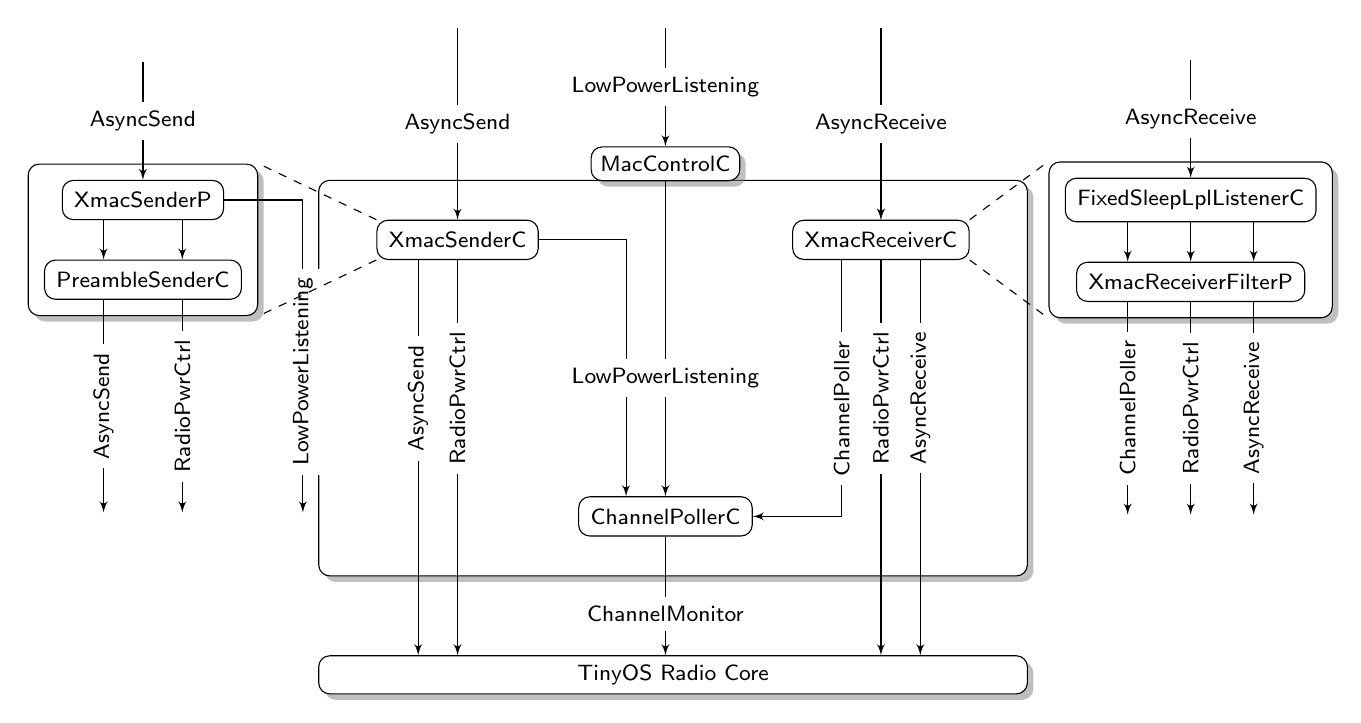
\begin{tikzpicture}
\tikzstyle{every node}=[font=\sffamily\footnotesize]

\node[layer, minimum width=9cm] (Core) { TinyOS Radio Core };

\node[layer, matrix, above=of Core, 
      column sep=5mm, row sep=30mm, inner sep=5mm,
      minimum width=9cm, nodes={reset, component}] (MacC) {
  \node (SenderC) {XmacSenderC}; & & \node (ReceiverC) {XmacReceiverC}; \\
  & \node (ChannelPollerC) {ChannelPollerC}; & \\
};

\node[layer, above=40mm of ChannelPollerC] (MacControlC) { MacControlC };

\node[layer, matrix, row sep=5mm, inner sep=2mm, nodes={reset, component}, 
  left=15mm of SenderC] (SenderDetail) {
  \node (XmacSenderP) { XmacSenderP }; \\
  \node (PreambleSenderC) { PreambleSenderC }; \\
};

\node[layer, matrix, row sep=5mm, inner sep=2mm, nodes={reset, component}, 
  right=10mm of ReceiverC] (ReceiverDetail) {
  \node (LplListenerC) { FixedSleepLplListenerC }; \\
  \node (RecvFilterP) { XmacReceiverFilterP }; \\
};


\coordinate[above=15mm of MacControlC] (Inputs) {};
\draw ([xshift=0mm] SenderC.south) coordinate (sout1) {};
\draw ([xshift=-5mm] SenderC.south) coordinate (sout2) {};

\draw ([xshift=0mm] ReceiverC.south) coordinate (rout1) {};
\draw ([xshift=5mm] ReceiverC.south) coordinate (rout2) {};

\coordinate[above=15mm of XmacSenderP] (xsin) {};
\coordinate[above=15mm of LplListenerC] (fslin) {};

\draw ([xshift=5mm] XmacSenderP.south) coordinate (xsout1) {};
\draw ([xshift=-5mm] XmacSenderP.south) coordinate (xsout2) {};
\draw ([xshift=10mm] XmacSenderP.east) coordinate (xsout3) {};

\draw ([xshift=8mm] LplListenerC.south) coordinate (fslout1) {};
\draw (LplListenerC.south) coordinate (fslout2) {};
\draw ([xshift=-8mm] LplListenerC.south) coordinate (fslout3) {};

\coordinate[below=27mm of PreambleSenderC] (psout) {};
\coordinate[below=27mm of RecvFilterP] (rcvout) {};

\draw ([xshift=-5mm] PreambleSenderC.south) coordinate (psout1) {};
\draw ([xshift=5mm] PreambleSenderC.south) coordinate (psout2) {};

\draw (RecvFilterP.south) coordinate (rcvout2) {};
\draw ([xshift=-8mm] RecvFilterP.south) coordinate (rcvout3) {};
\draw ([xshift=8mm] RecvFilterP.south) coordinate (rcvout1) {};


\draw[->] (Inputs) -- (MacControlC) node [midway, fill=white] { LowPowerListening };
\draw[->] (MacControlC) -- (MacControlC |- ChannelPollerC.north);
\draw[->] (SenderC) -| ([xshift=-5mm] ChannelPollerC.north);
%\draw[->] (ReceiverC) -| ([xshift=5mm] ChannelPollerC.north);
\draw[->] ([xshift=-5mm] ReceiverC.south) |- (ChannelPollerC.east) 
           node [pos=0.29, fill=white, rotate=90] { ChannelPoller };
\node[fill=white] at ([yshift=-25mm] MacControlC.south) (LPL) { LowPowerListening };
\draw[->] (ChannelPollerC.south) -- (MacControlC |- Core.north) 
           node [pos=0.65, fill=white] { ChannelMonitor };

\draw[->] (Inputs -| SenderC) -- (SenderC) node [midway, fill=white] { AsyncSend };
\draw[->] (sout1) -- (sout1 |- Core.north) node [pos=0.35, fill=white, rotate=90] { RadioPwrCtrl };
\draw[->] (sout2) -- (sout2 |- Core.north) node [pos=0.35, fill=white, rotate=90] { AsyncSend };

\draw[->] (xsin) -- (XmacSenderP) node [midway, fill=white] { AsyncSend };
\draw[->] (xsout1) -- (xsout1 |- PreambleSenderC.north);
\draw[->] (xsout2) -- (xsout2 |- PreambleSenderC.north);
\draw[->] (psout1) -- (psout1 |- psout) node [midway, fill=white, rotate=90] { AsyncSend };
\draw[->] (psout2) -- (psout2 |- psout) node [midway, fill=white, rotate=90] { RadioPwrCtrl };
\draw[->] (XmacSenderP.east) -- (xsout3) -- (xsout3 |- psout)
          node[pos=0.55, fill=white, rotate=90] { LowPowerListening };


\draw[->] (Inputs -| ReceiverC) -- (ReceiverC) node [midway, fill=white] { AsyncReceive };
\draw[->] (rout1) -- (rout1 |- Core.north) node [pos=0.35, fill=white, rotate=90] { RadioPwrCtrl };
\draw[->] (rout2) -- (rout2 |- Core.north) node [pos=0.35, fill=white, rotate=90] { AsyncReceive };

\draw[->] (fslin) -- (LplListenerC) node [midway, fill=white] { AsyncReceive };
\draw[->] (fslout1) -- (fslout1 |- RecvFilterP.north);
\draw[->] (fslout2) -- (fslout2 |- RecvFilterP.north);
\draw[->] (fslout3) -- (fslout3 |- RecvFilterP.north);
\draw[->] (rcvout1) -- (rcvout1 |- rcvout) node [midway, fill=white, rotate=90] { AsyncReceive };
\draw[->] (rcvout2) -- (rcvout2 |- rcvout) node [midway, fill=white, rotate=90] { RadioPwrCtrl };
\draw[->] (rcvout3) -- (rcvout3 |- rcvout) node [midway, fill=white, rotate=90] { ChannelPoller };

\draw[->] (Inputs -| ReceiverC) -- (ReceiverC) node [midway, fill=white] { AsyncReceive };

\draw[dashed] (SenderC.north west) -- (SenderDetail.north east);
\draw[dashed] (SenderC.south west) -- (SenderDetail.south east);

\draw[dashed] (ReceiverC.north east) -- (ReceiverDetail.north west);
\draw[dashed] (ReceiverC.south east) -- (ReceiverDetail.south west);

\end{tikzpicture}
%\end{document}
